\documentclass[12pt,a4paper]{article}
\usepackage{fontspec}
\setmainfont{DejaVu Serif}
\setsansfont{DejaVu Sans}
\setmonofont{DejaVu Sans Mono}
\usepackage{babel}
\babelprovide[main,import]{russian}
\usepackage{amsmath, amssymb, amsthm}
\usepackage{graphicx}
\usepackage{hyperref}
\usepackage{listings}
\usepackage{xcolor}
\usepackage{geometry}
\usepackage{float}
\usepackage{caption}
\usepackage{subcaption}
\usepackage{enumitem}
\usepackage{titlesec}
\usepackage{fancyhdr}
\usepackage{array}
\usepackage{longtable}
\usepackage{booktabs}

% Настройка полей
\geometry{
    a4paper,
    left=2.5cm,
    right=1.5cm,
    top=2cm,
    bottom=2cm
}

% Настройка заголовков
\titleformat{\section}{\Large\bfseries}{\thesection}{1em}{}
\titleformat{\subsection}{\large\bfseries}{\thesubsection}{1em}{}
\titleformat{\subsubsection}{\normalsize\bfseries}{\thesubsubsection}{1em}{}

% Настройка кода
\lstset{
    language=Python,
    basicstyle=\ttfamily\small,
    keywordstyle=\color{blue},
    commentstyle=\color{green!40!black},
    stringstyle=\color{red},
    numbers=left,
    numberstyle=\tiny,
    breaklines=true,
    frame=single,
    captionpos=b,
    showstringspaces=false,
    tabsize=4
}

% Настройка колонтитулов
\pagestyle{fancy}
\fancyhf{}
\fancyhead[L]{Лабораторная работа: Проектирование AI-сервиса на FastAPI}
\fancyhead[R]{\thepage}
\fancyfoot[C]{}


\usepackage{tabularx}
\usepackage{xurl}
\sloppy
\usepackage{tikz}
\usetikzlibrary{arrows.meta,positioning}
\setlength{\headheight}{30pt}
\setlength{\emergencystretch}{3em}
\hypersetup{hidelinks}
\renewcommand{\lstlistingname}{Листинг}
\lstset{columns=fullflexible,keepspaces=true,basicstyle=\ttfamily\footnotesize}
% Замените значением URL вашего проекта после загрузки кода на GitHub.
\newcommand{\RepositoryURL}{}
\newcommand{\StudentName}{Сульповар Михаил Леонидович}
\newcommand{\StudentGroup}{МПИ-25-1-1}
\newcommand{\TeacherName}{\underline{\hspace{5cm}}}
\begin{document}

\begin{titlepage}
    \begin{center}
        \textbf{МИНИСТЕРСТВО НАУКИ И ВЫСШЕГО ОБРАЗОВАНИЯ РОССИЙСКОЙ ФЕДЕРАЦИИ}
        \vspace{0.5cm}
        
        \textbf{Федерального государственного автономного образовательного учреждения \\ высшего образования}
        \vspace{0.3cm}
        
        \textbf{«НАЦИОНАЛЬНЫЙ ИССЛЕДОВАТЕЛЬСКИЙ ТЕХНОЛОГИЧЕСКИЙ УНИВЕРСИТЕТ МИСИС»}
        \vspace{2cm}

        
        \textbf{Институт компьютерных наук}
        \vspace{0.3cm}

        \textbf{Кафедра Инженерной кибернетики}
        \vspace{1cm}
        
        \textbf{Лабораторная работа №1}
        \vspace{0.3cm}
        
        \textbf{по дисциплине «Современные интеллектуальные сетевые сервисы»}
        \vspace{1.5cm}
        
        \huge{\textbf{Проектирование AI-сервиса \\ на FastAPI}}
        \vspace{2cm}
    \end{center}
    
    \begin{flushright}
        \textbf{Выполнил:} \\
        Студент группы \StudentGroup \\
        \StudentName \\
        \vspace{0.5cm}
        \textbf{Проверил:} \\
        Преподаватель \\
        \TeacherName \\
        \vspace{2cm}
        \textbf{Оценка:} \hrulefill
    \end{flushright}
    
    \begin{center}
        \vfill
        Москва, 2026
    \end{center}
\end{titlepage}


\tableofcontents
\newpage

\section{Цель работы}
Научиться проектировать программную архитектуру AI-сервиса, определить место API в общей интеллектуальной системе и реализовать REST API на FastAPI. Освоить передачу JSON, входные и выходные схемы Pydantic, структурную и бизнес-валидацию, HTTP-коды, хранение результатов и описание контракта OpenAPI.

\section{Краткое описание архитектуры API}
Разработан сервис Agro Scoring API для оценки риска сельскохозяйственного предприятия. Потребители: CRM банка, веб-портал, мобильное приложение, внутренние банковские сервисы и BI-система. Обмен выполняется по HTTP в формате JSON; для внешнего развертывания требуется HTTPS.

В работе используется учебная модель на правилах, а не обученная ML-модель. Прогноз возвращается синхронно в рамках одного запроса. Длительные операции (обучение модели, пакетный инференс) в прототип не включены: в дальнейшем им потребуется очередь задач и отдельный обработчик. Асинхронная функция middleware обслуживает HTTP-запросы, но сама по себе не делает инференс фоновой задачей.

\subsection{Программные компоненты}
Ответственности разделены по директориям без микросервисов и дополнительных фреймворков.
\begin{table}[H]
\centering\caption{Компоненты приложения}
\begin{tabularx}{\textwidth}{|p{5.1cm}|X|}\hline
\textbf{Файл} & \textbf{Ответственность} \\\hline
\path{app/main.py} & Сборка FastAPI, подключение маршрутов, логирование, middleware времени обработки. \\\hline
\path{app/api/routes.py} & HTTP-методы, path/query-параметры, статусы и преобразование исключений сервиса. \\\hline
\texttt{app/schemas/}\newline\texttt{prediction.py} & Входные и выходные модели Pydantic, ограничения полей. \\\hline
\path{app/models/risk.py} & Расчет риска и метаданные учебной модели. \\\hline
\texttt{app/services/}\newline\texttt{scoring.py} & Бизнес-валидация, инференс, постпроцессинг и сохранение результата. \\\hline
\texttt{app/repositories/}\newline\texttt{predictions.py} & Хранилище прогнозов и выборка последних результатов. \\\hline
\end{tabularx}
\end{table}

\subsection{Компонентная схема}
\begin{figure}[H]
\centering
\begin{tikzpicture}[
box/.style={draw,rounded corners,align=center,text width=4.1cm,minimum height=1cm,font=\small},
arrow/.style={-{Stealth},thick},node distance=0.9cm]
\node[box,text width=13cm] (clients) {CRM, веб-портал, мобильное приложение, BI};
\node[box,below=of clients,text width=8cm] (api) {HTTP / JSON: FastAPI\\main.py, api/routes.py; middleware, статусы};
\node[box,below=of api] (service) {services/scoring.py\\бизнес-валидация\\и постпроцессинг};
\node[box,left=0.4cm of service] (schema) {schemas/\\prediction.py\\контракт Pydantic};
\node[box,right=0.4cm of service] (storage) {repositories/\\predictions.py\\результаты в памяти};
\node[box,below=of service] (model) {models/risk.py\\учебная модель};
\draw[arrow] (clients)--(api);
\draw[arrow] (schema.north)|-(api.west);
\draw[arrow] (api)--(service);
\draw[arrow] (service)--(storage);
\draw[arrow] (service)--(model);
\end{tikzpicture}
\caption{Компонентная схема сервиса агроскоринга}
\end{figure}

\subsection{Входные и выходные данные}
Все девять полей запроса обязательны. Строки очищаются от пробелов по краям; пустые значения не допускаются. Числовые значения должны быть конечными.
\begin{table}[H]
\centering\caption{Ограничения входных данных}
\begin{tabularx}{\textwidth}{|p{5cm}|p{2cm}|X|}\hline
Поле & Тип & Ограничение \\\hline
\texttt{farm\_id}, \texttt{region}, \texttt{crop\_type} & string & Не менее одного символа после удаления внешних пробелов. \\\hline
\texttt{area\_ha} & number & Больше нуля. \\\hline
\texttt{temperature\_avg} & number & От $-60$ до $60$ включительно. \\\hline
\texttt{precipitation\_mm}, \texttt{debt} & number & Не меньше нуля. \\\hline
\texttt{payment\_delay\_days}, \texttt{previous\_defaults} & integer & Не меньше нуля. \\\hline
\end{tabularx}
\end{table}
Регион дополнительно проверяется по справочнику \texttt{Krasnodar}, \texttt{Rostov}, \texttt{Stavropol}. Ответ включает \texttt{request\_id}, \texttt{farm\_id}, \texttt{risk\_score}, \texttt{risk\_level}, \texttt{recommendation}, \texttt{model\_version}.

\subsection{Контур инференса и небольшое изменение логики}
Последовательность обработки запроса:
\begin{enumerate}
\item Pydantic проверяет тело запроса до вызова обработчика; нарушение контракта дает 422.
\item Сервис проверяет готовность модели; если она недоступна, возвращается 503.
\item Регион проверяется по бизнес-справочнику; неизвестный регион дает 400.
\item Создается UUID4 и записывается начало обработки в журнал.
\item Вычисляется оценка риска, категория и рекомендация.
\item Прогноз сохраняется в хранилище; результат обработки записывается в журнал.
\item Возвращается 201 и заголовок \texttt{Location} с путем созданного прогноза.
\end{enumerate}
Исходная логика сохранена. Единственное дополнение к расчету: средняя температура ниже $5\,^{\circ}\mathrm{C}$ или выше $35\,^{\circ}\mathrm{C}$ увеличивает оценку на $0{,}05$. Это условное учебное правило, его эффективность на реальных данных не проверялась. Версия модели изменена на 1.1.
\begin{table}[H]
\centering\caption{Правила расчета риска}
\begin{tabularx}{\textwidth}{|X|c|}\hline
Условие & Вклад \\\hline
Базовая оценка & 0,10 \\\hline
Просрочка больше 30 дней & +0,30 \\\hline
Есть хотя бы один предыдущий дефолт & +0,30 \\\hline
Задолженность больше 5 000 000 & +0,20 \\\hline
Осадки меньше 100 мм & +0,10 \\\hline
Средняя температура ниже 5 или выше 35 градусов & +0,05 \\\hline
\end{tabularx}
\end{table}
Сумма ограничивается сверху единицей и округляется до двух знаков. Категории: \texttt{low} при $s<0{,}3$, \texttt{medium} при $0{,}3\leq s<0{,}7$, \texttt{high} при $s\geq0{,}7$. Рекомендации: стандартное рассмотрение, дополнительная проверка, ручное рассмотрение соответственно.

\subsection{Хранение, наблюдаемость и ограничения}
Результаты хранятся в словаре одного экземпляра приложения. Блокировка защищает запись и создание снимка словаря при параллельных запросах. Список возвращается в обратном порядке сохранения: сначала новые результаты. Фильтрация выполняется до ограничения количества.

Middleware добавляет \texttt{X-Process-Time} в секундах и записывает метод, путь, статус и длительность. Журнал успешного инференса содержит идентификаторы запроса и хозяйства, оценку и категорию риска. Полное тело запроса в журнал не записывается.

При перезапуске данные теряются; несколько процессов имеют независимые хранилища. Память растет с числом прогнозов. Для дальнейшего развития нужны БД, политика удаления старых записей, аутентификация, контроль доступа и проверка качества настоящей модели. В учебном запуске используется один процесс. Обученную модель можно подключить в модуле модели; подключение БД потребует адаптации хранилища и сборки приложения при сохранении HTTP-контракта.

\section{Исходный код приложения}
\if\relax\detokenize\expandafter{\RepositoryURL}\relax
\textbf{Ссылка на проект:} добавляется после загрузки проекта в собственный репозиторий. Перед сдачей необходимо заполнить команду \texttt{\textbackslash RepositoryURL} в начале этого файла.
\else
\textbf{Ссылка на проект:} \expandafter\url\expandafter{\RepositoryURL}.
\fi
Код поставляется в архиве \texttt{agro\_scoring.zip}. Директории отражают отдельные ответственности, импорты идут от корневого пакета \texttt{app}. Нет циклических импортов между API и сервисом.
\begin{lstlisting}[language={},caption={Структура проекта}]
agro_scoring/
    app/
        main.py
        api/routes.py
        schemas/prediction.py
        models/risk.py
        services/scoring.py
        repositories/predictions.py
    tests/test_api.py
    requirements.txt
    requirements-dev.txt
    pyproject.toml
    README.md
    report/
        main.tex
        images/
\end{lstlisting}
В директориях Python также находятся \texttt{\_\_init\_\_.py}. Проверка стиля: Ruff, длина строки 88, правила E/W/F/I/UP/B/SIM. Докстринги написаны в свободной форме. Для запуска нужен Python 3.12 или новее.
\begin{lstlisting}[language={},caption={Установка, запуск и проверка из корня проекта}]
python -m pip install -r requirements-dev.txt
python -m uvicorn app.main:app --reload
python -m pytest -q
python -m ruff check .
python -m ruff format --check .
\end{lstlisting}
Для обычного запуска достаточно \texttt{requirements.txt}; зависимости тестов и Ruff находятся в \texttt{requirements-dev.txt}. LaTeX собирается XeLaTeX дважды из директории \texttt{report}; используются шрифты DejaVu и изображения из \texttt{images}.

\section{Реализованные endpoints}
\begin{table}[H]
\centering\caption{Маршруты API}
\begin{tabularx}{\textwidth}{|l|p{5.6cm}|X|}\hline
Метод & Endpoint & Назначение \\\hline
GET & \texttt{/health} & Доступность процесса API. \\\hline
GET & \texttt{/model-info} & Метаданные и состояние модели. \\\hline
POST & \texttt{/predict} & Создание и сохранение прогноза. \\\hline
GET & \texttt{/predictions/}\newline\texttt{\{request\_id\}} & Чтение результата по ID. \\\hline
GET & \texttt{/predictions} & Последние прогнозы с фильтрацией. \\\hline
\end{tabularx}
\end{table}
\subsection{Чем /health отличается от /model-info?}
\texttt{/health} возвращает \texttt{\{"status": "ok"\}} и проверяет доступность API. \texttt{/model-info} описывает модель и возвращает состояние \texttt{ready} или \texttt{unavailable}. API может отвечать на запросы, когда модель недоступна; тогда корректный запрос \texttt{/predict} получает 503.

\subsection{Почему некорректный запрос не должен доходить до модели?}
Отрицательная площадь физически невозможна. Такие признаки нарушают ожидаемый формат данных, могут вызвать ошибку вычислений или недостоверный результат. Валидация предотвращает бесполезный инференс и сохранение ошибочного прогноза; клиент получает указание на конкретное поле. Бизнес-валидатор отдельно отклоняет формально корректный, но неподдерживаемый регион.

\subsection{Выбор между 200 и 201}
Выбран 201 Created: каждый успешный запрос создает новый сохраненный прогноз с UUID. Заголовок \texttt{Location} указывает его адрес. Все операции чтения возвращают 200. Для инференса без создания сохраняемого ресурса можно было бы выбрать 200, но в этой реализации семантика создания используется последовательно.

\section{Swagger UI}
Документация доступна по адресу \url{http://127.0.0.1:8000/docs}, спецификация по \url{http://127.0.0.1:8000/openapi.json}. Swagger показывает маршруты, схемы, ограничения и ответы. Значения фильтра категории описаны типом \texttt{Literal}; некорректная категория дает 422.
\begin{figure}[H]\centering
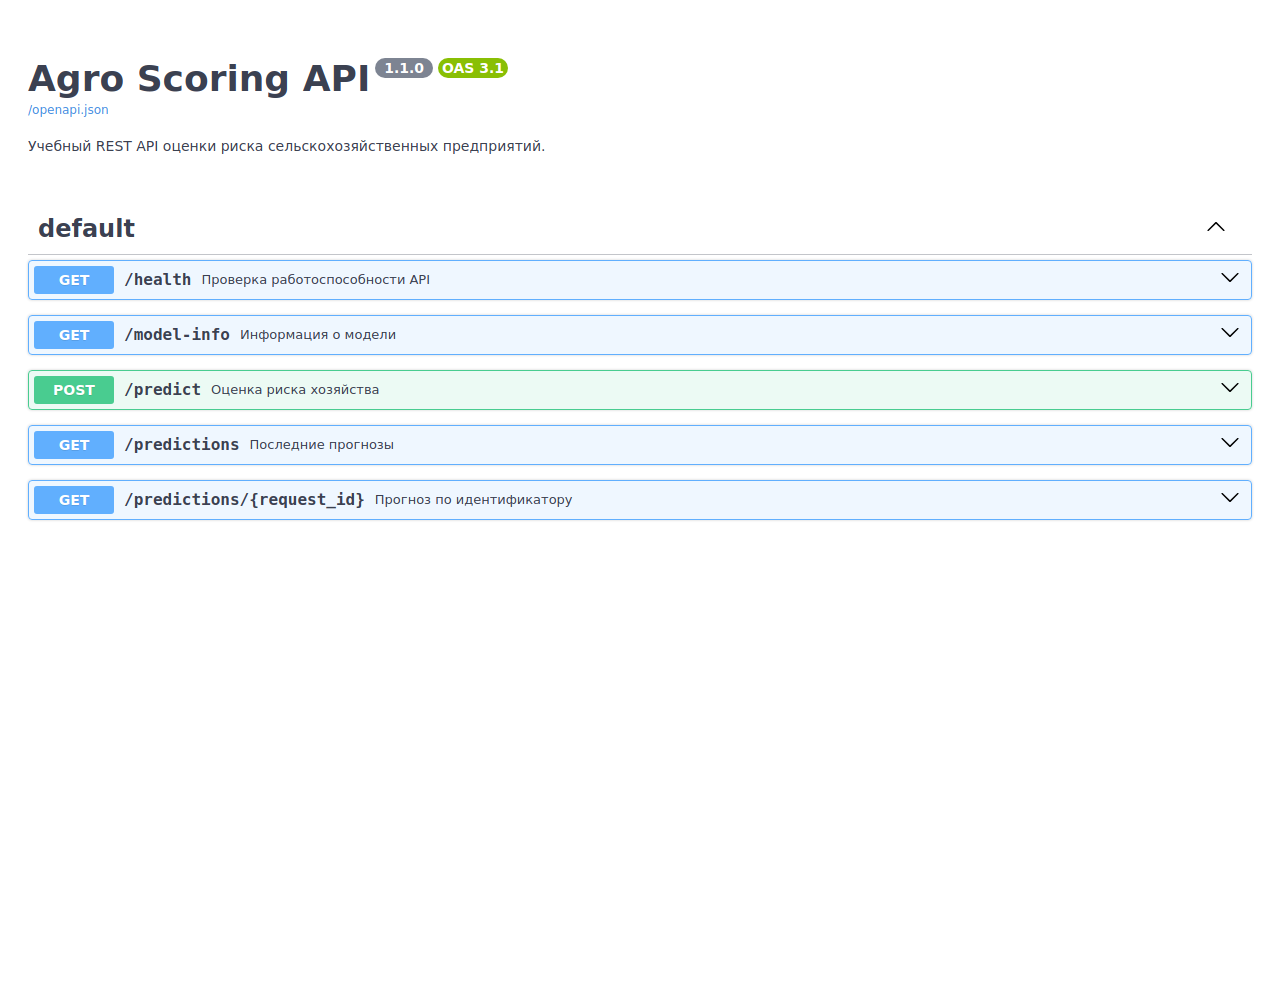
\includegraphics[width=\textwidth,height=0.72\textheight,keepaspectratio]{images/swagger.png}
\caption{Swagger UI работающего приложения}
\end{figure}

\section{Успешный запрос /predict}
\lstinputlisting[language={},caption={Тело запроса}]{request.json}
Для выбранных данных сумма составляет $0{,}10+0{,}30+0{,}30+0{,}20+0{,}10+0{,}05=1{,}05$. После ограничения получено 1,00, категория \texttt{high}, рекомендация ручного рассмотрения.
\begin{figure}[H]\centering
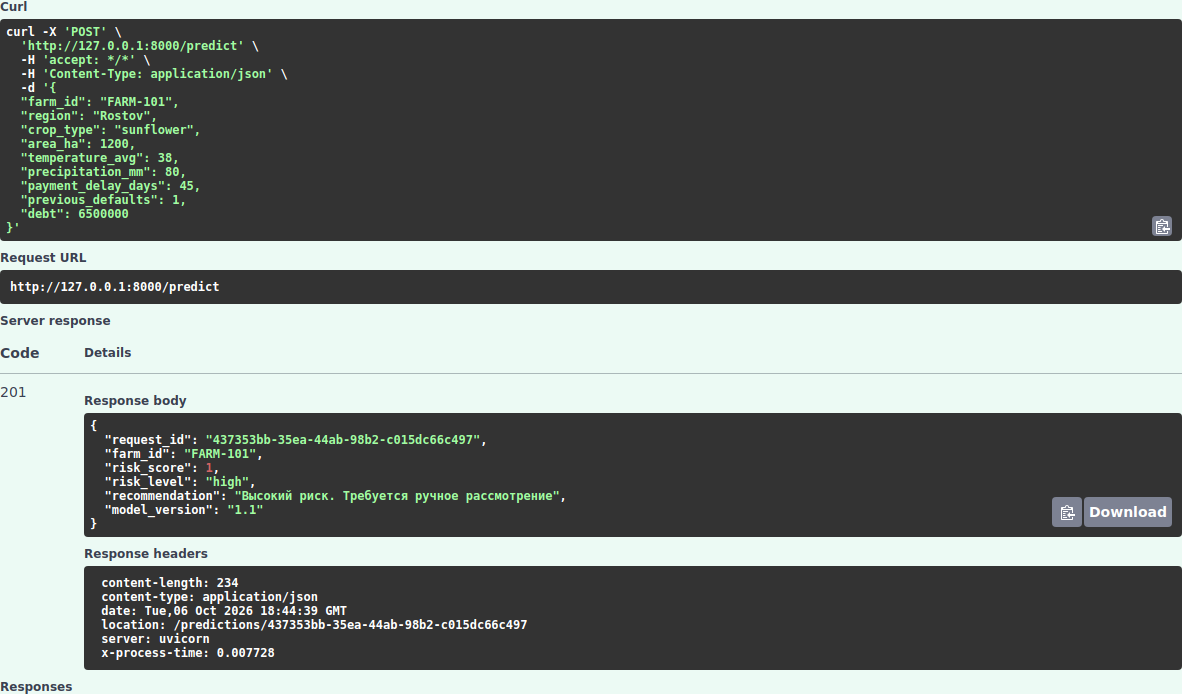
\includegraphics[width=\textwidth,height=0.72\textheight,keepaspectratio]{images/success.png}
\caption{Успешное выполнение POST /predict в Swagger UI, HTTP 201}
\end{figure}
UUID создается при каждом запросе; он не фиксирован в программе.

\section{Ошибка валидации Pydantic}
В исходном запросе площадь заменена на $-100$. Получен 422, модель не вызывается и результат не сохраняется. Массив \texttt{detail} содержит тип нарушения, положение поля, сообщение, исходное значение и ограничение.
\lstinputlisting[language={},caption={Ответ Pydantic на отрицательную площадь}]{validation.json}
\begin{figure}[H]\centering
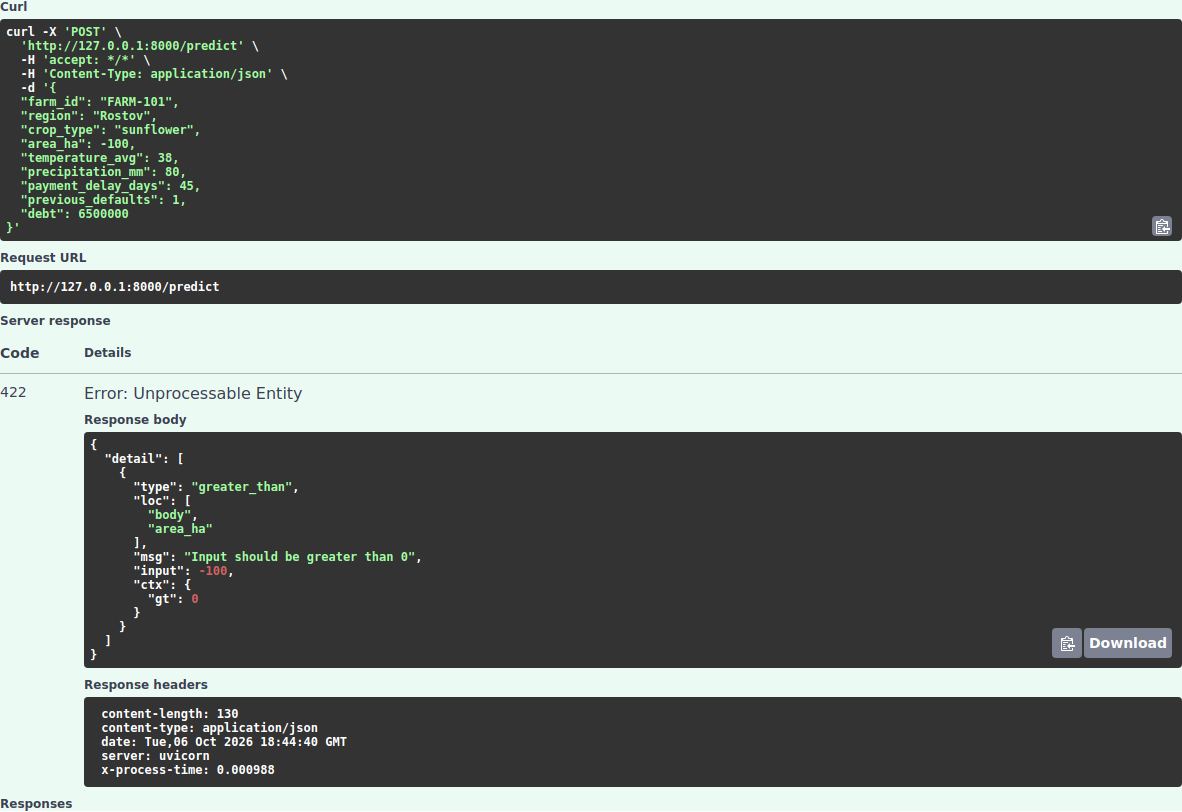
\includegraphics[width=\textwidth,height=0.72\textheight,keepaspectratio]{images/validation.png}
\caption{Ошибка структурной валидации в Swagger UI, HTTP 422}
\end{figure}

\section{Ошибка 404 Not Found}
Выполнен запрос к \texttt{/predictions/unknown-id}. Такого идентификатора в хранилище нет; ответ содержит \texttt{detail: Prediction not found}.
\begin{figure}[H]\centering
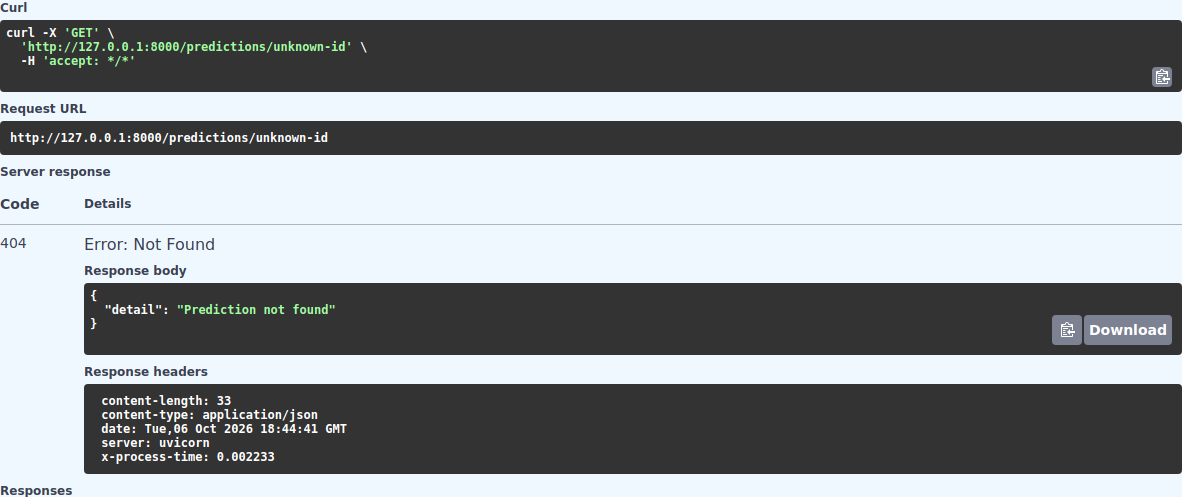
\includegraphics[width=\textwidth,height=0.72\textheight,keepaspectratio]{images/not_found.png}
\caption{Обращение к отсутствующему прогнозу в Swagger UI, HTTP 404}
\end{figure}

\section{Таблица тест-кейсов}
Проверки выполнены с помощью FastAPI TestClient. Все строки таблицы получены при фактическом выполнении запросов. Дополнительно набор pytest проверяет порядок результатов, фильтрацию, сохранение, заголовки, границы категорий, температурное правило и OpenAPI: 22 проверки пройдены.
\begin{table}[H]
\centering\caption{Результаты HTTP-проверок}
\small
\begin{tabularx}{\textwidth}{|c|X|c|c|c|}\hline
№ & Запрос / условие & Ожидалось & Получено & Итог \\\hline
1 & GET /health & 200 & 200 & OK \\
2 & GET /model-info & 200 & 200 & OK \\
3 & Корректный POST /predict & 201 & 201 & OK \\
4 & area\_ha = -100 & 422 & 422 & OK \\
5 & Неизвестный регион & 400 & 400 & OK \\
6 & Существующий request\_id & 200 & 200 & OK \\
7 & Неизвестный request\_id & 404 & 404 & OK \\
8 & limit = 2 & 200 & 200 & OK \\
9 & risk\_level = high & 200 & 200 & OK \\
10 & limit = -5 & 422 & 422 & OK \\
11 & limit = 101 & 422 & 422 & OK \\
12 & risk\_level = extreme & 422 & 422 & OK \\
13 & risk\_level = medium, limit = 5 & 200 & 200 & OK \\
14 & Отсутствует поле debt & 422 & 422 & OK \\
15 & Модель недоступна & 503 & 503 & OK \\

\hline
\end{tabularx}
\end{table}
Ruff check и Ruff format --check выполнены успешно. При тестировании использовались версии зависимостей, зафиксированные в файлах требований.

\section{Таблица API-контракта}
\begin{table}[H]
\centering\caption{Контракт API}
\scriptsize
\begin{tabularx}{\textwidth}{|p{3.6cm}|l|p{3.3cm}|X|c|p{1.5cm}|}\hline
Endpoint & Метод & Вход & Выход & Успех & Ошибки \\\hline
\texttt{/health} & GET & Нет & HealthResponse & 200 & 500 \\\hline
\texttt{/model-info} & GET & Нет & ModelInfoResponse & 200 & 500 \\\hline
\texttt{/predict} & POST & JSON: FarmRequest & PredictionResponse & 201 & 400, 422, 503, 500 \\\hline
\texttt{/predictions/}\newline\texttt{\{request\_id\}} & GET & path: request\_id & PredictionResponse & 200 & 404, 422, 500 \\\hline
\texttt{/predictions} & GET & query: limit, risk\_level & Массив PredictionResponse & 200 & 422, 500 \\\hline
\end{tabularx}
\end{table}
Параметр \texttt{limit}: целое число от 1 до 100, по умолчанию 10. \texttt{risk\_level}: необязательный фильтр \texttt{low}, \texttt{medium}, \texttt{high}. Path-параметр \texttt{request\_id} имеет тип строки; произвольный отсутствующий идентификатор возвращает 404. Код 422 для path-маршрута присутствует в автоматически создаваемой спецификации FastAPI; отдельное UUID-ограничение не введено.

Бизнес-ошибки 400, 404 и 503 явно описаны через \texttt{responses} и схему ErrorResponse. Ошибки валидации 422 добавляются FastAPI автоматически. Код 500 указан как возможный непредвиденный серверный сбой, а не как штатный бизнес-ответ; его отдельная схема в OpenAPI не объявлялась.

\section{Вывод}
Разработан и проверен учебный AI-сервис агроскоринга. Сборка приложения, HTTP-маршруты, контракт данных, модель, бизнес-логика и хранилище разделены по самостоятельным модулям. Структурная и бизнес-валидация выполняются до инференса; прогноз сохраняется под UUID и доступен повторно. Реализованы пять обязательных endpoints, корректные HTTP-коды, фильтрация, выдача последних результатов, логирование и измерение времени обработки.

REST API служит общей точкой входа для потребителей, фиксирует контракт и скрывает внутреннюю реализацию модели. Благодаря разделению ответственностей модель и способ хранения можно развивать при сохранении клиентского интерфейса. Прототип остается ограниченным учебным решением: модель является набором правил, результаты хранятся только в памяти одного процесса.

\end{document}
